\chapter{Introduction}

Here begins with the introduction. And a citation test \cite{Batley2015}

\section{An example of a section within a chapter}
\subsection{An example of a subsection}

\begin{figure}[t]
\centering
  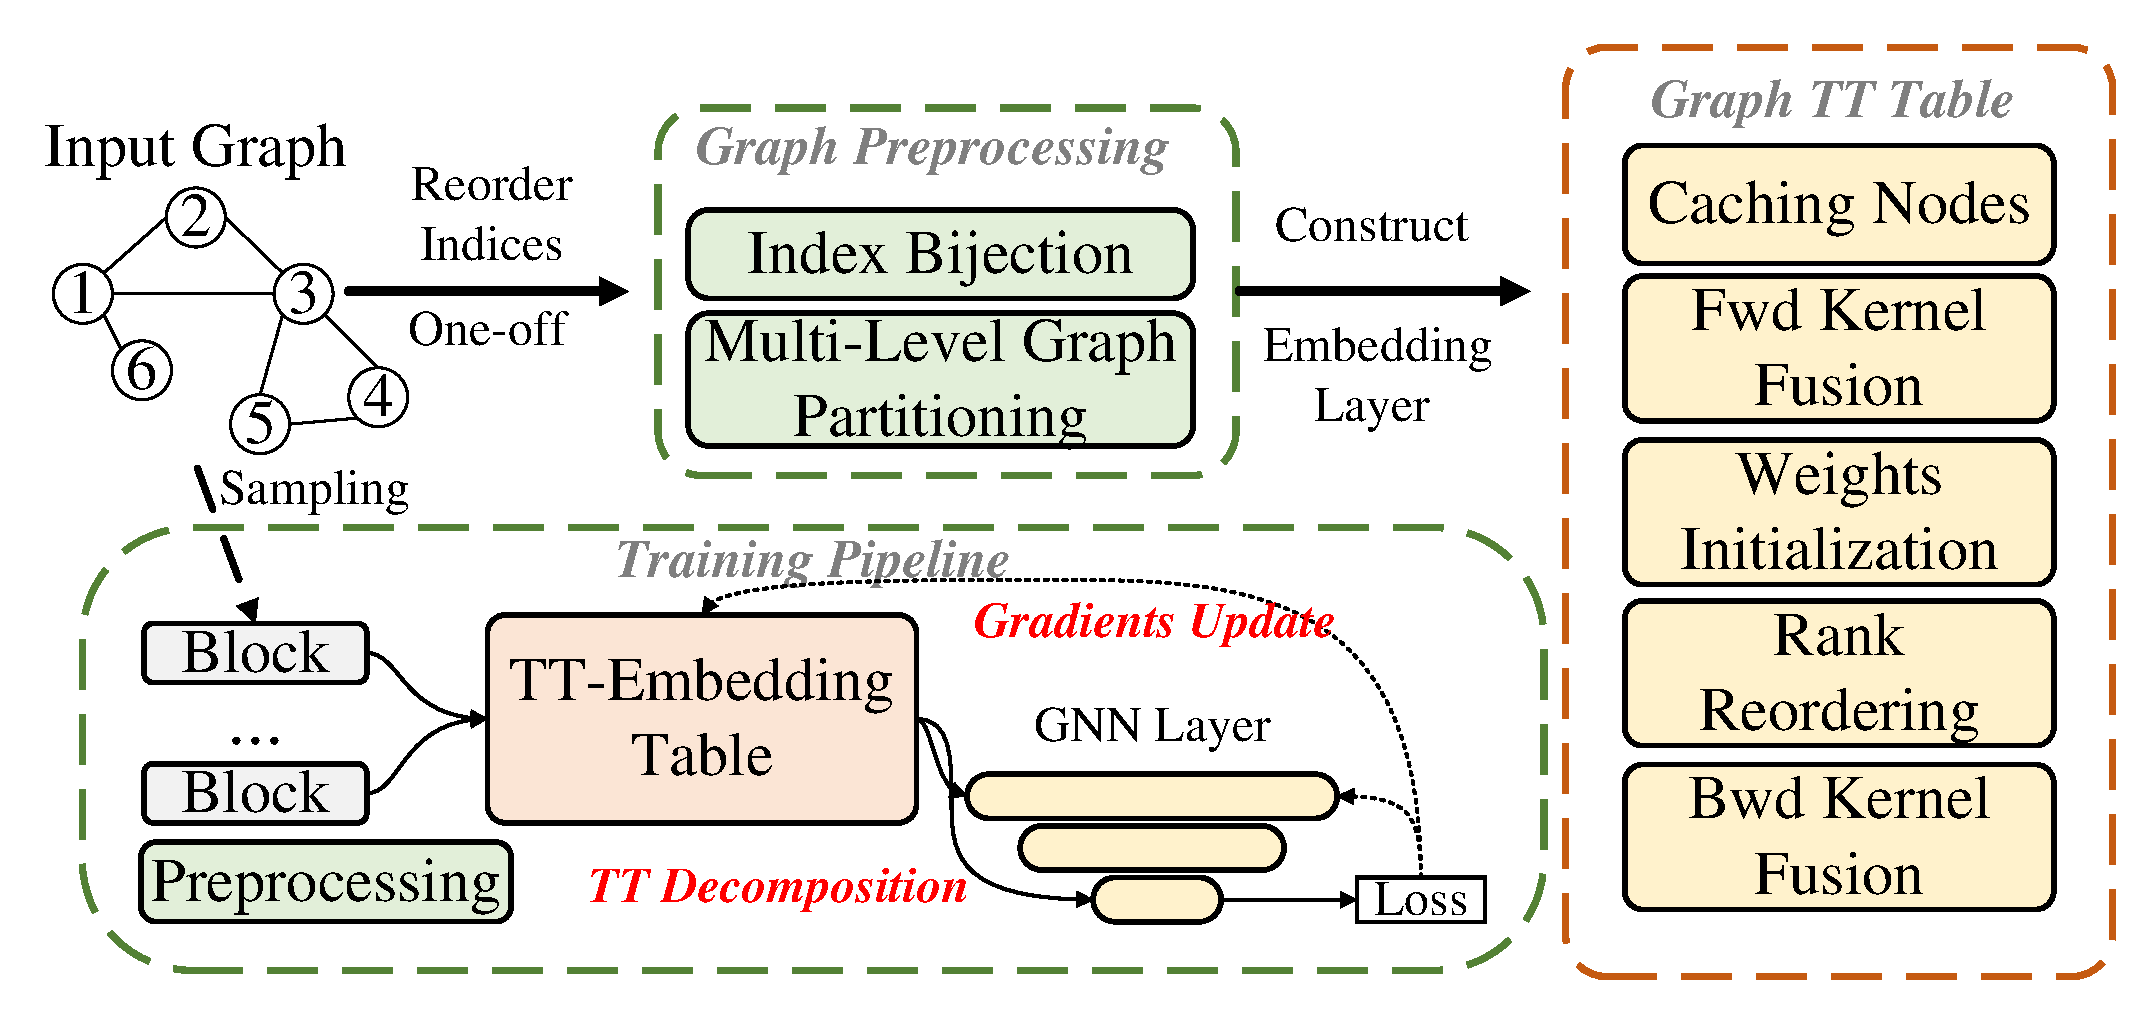
\includegraphics[width=\columnwidth]{Figures/overview.pdf}
\caption{ a \sys overview}
\label{fig:overview}
\end{figure}

\begin{table}[t]
\centering
\footnotesize
\caption{A table example v1}
\rowcolors{2}{white}{gray!13}
\begin{tabularx}{\columnwidth}{XXX}
\toprule
\textbf{Approach} & \textbf{Acc. (\%)}  & \textbf{Speedup} \\ 
\midrule
\multicolumn{3}{c}{Train with dataset X1} \\ 
\hline
Mortal           & 66.2        & 1x \\ 
Elf              & 64.8        & 2x \\ 
\sys             & 65.7        & 5x \\ 
\hline
\multicolumn{3}{c}{Train with dataset X2}  \\ 
\hline
Mortal           & 66.2        & 1x \\ 
Elf              & 64.8        & 2x \\ 
\sys             & 65.7        & 5x \\ 
\hline
\multicolumn{3}{c}{Train with dataset x3} \\ 
\hline
Mortal           & 66.2        & 1x \\ 
Elf              & 64.8        & 2x \\ 
\sys             & 65.7        & 5x \\ 
\bottomrule
\end{tabularx}
\label{tab:table_ex1}
\end{table}

\begin{table}
	\begin{center}
\begin{tabular}{ |p{3cm}||p{3cm}|p{3cm}|p{3cm}|  }
	\hline
	\multicolumn{4}{|c|}{Country List} \\
	\hline
	Country Name     or Area Name& ISO ALPHA 2 Code &ISO ALPHA 3 Code&ISO numeric Code\\
	\hline
	Afghanistan   & AF    &AFG&   004\\
	Aland Islands&   AX  & ALA   &248\\
	Albania &AL & ALB&  008\\
	Algeria    &DZ & DZA&  012\\
	American Samoa&   AS  & ASM&016\\
	Andorra& AD  & AND   &020\\
	Angola& AO  & AGO&024\\
	\hline
\end{tabular}
\caption{A table example v2 taken from \url{https://www.overleaf.com/}. Make sure the label goes after the caption for figures and tables!}
\label{tab:table_ex2}
\end{center}	
\end{table}


\begin{algorithm} [t]
\footnotesize
  \SetAlgoLined
  \DontPrintSemicolon
  \caption{A showing example: Tensor-Train Decomposition in Graph Embeddings}
  \KwIn{Embedding Tensor $\mathcal{W} \in \mathbb{R}^{M \times N}$}
  \KwOut{Tensor train cores $\mathcal{G}_1, \mathcal{G}_2, \dots \mathcal{G}_d$ }
  \tcp{Initialization}
  $\mathcal{W}$ = reshape([$p_1, p_2, \dots, p_d$, $q_1, q_2, \dots, q_k$, $q_d$]) \;
  temp = transpose($\mathcal{W}$, [$p_1, q_1, p_2, q_2, \dots, p_d, q_d$]) \;
  \For{(i=0; i<d; i++)} {
    temp = reshape([$r_i * p_i * q_i$,:]) \;
    \tcp{A TT SVD follows: temp $= U \Sigma V^T + E$}
    temp = TT\_SVD() \; 
    $\mathcal{G}_d$ = reshape(U, [$r_i, p_i, q_i, p_{i+1}$]) \;
  }
  $\mathcal{G}_d$ = reshape(temp, [$r_d, p_d, q_d, 1$]) \;
  return ($\mathcal{G}_1, \mathcal{G}_2, \dots \mathcal{G}_d$) \;
  \label{alg:example}
\end{algorithm}










